%Root main.tex
%---------------------------------------------------------------------------
%第1章　研究背景・目的
%---------------------------------------------------------------------------

\chapter{はじめに}
\label{chap:first}

\section{研究背景}
\subsection{系統連系システム}
日本は，すぐに使える資源に乏しく，国土を山と深い海に囲まれるなどの地理的制約を抱えており，
過去に幾度もエネルギー安定供給の危機に見舞われ，その都度，英知を結集してエネルギー安定供給の確保に取り組んできた．
しかし，2011年の東日本大震災および東京電力福島第一原子力発電所事故以降，原子力発電所の多くが停止した結果，
化石燃料に対する依存が高まり，その大宗を海外からの輸入に頼るという，エネルギー需給構造上の脆弱性が再び顕在化することとなった．

こうした中，2022年2月には，ロシアによるウクライナ侵略が発生し，日本を取り巻くエネルギー情勢は一変している．
エネルギー分野におけるインフレーションが世界的に顕著となり，国内でも電力需給ひっ迫やエネルギー価格の高騰が生じるなど，
石油危機以来のエネルギー危機が危惧される事態となった．
また2023年には，日本が原油の9割以上を依存する中東地域における軍事的な緊張が高まり，
化石燃料の調達に関する不確実性が上昇するなど，日本が抱えるエネルギー需給構造上の課題が改めて浮き彫りとなった．

エネルギーは国民生活や経済活動の基盤となるものであり，エネルギー安定供給が損なわれることは決してあってはならない．
化石燃料への過度な依存から脱却し，エネルギー危機にも耐え得るエネルギー需給構造への転換を進めていくためにも，
エネルギー安全保障に重点を置いた政策の再構築を進めることが強く求められている．

同時に，世界的な異常気象や大規模な自然災害が発生する中，世界では多くの国・地域が期限付きのカーボンニュートラル目標を表明し，
脱炭素に向けた機運は高い状態にある．こうした中，日本では，世界全体での1.5℃目標と整合的で，
2050年ネット・ゼロの実現に向けた直線的な経路にある野心的な目標として，
2035年度，2040年度に温室効果ガスを2013年度からそれぞれ60[\%]，73[\%]削減することを目指す新たな温室効果ガス削減目標を2025年2月に決定し，
気候変動問題に対して国家を挙げて対応する強い決意を表明した．\cite{ref00}．

再生可能エネルギーとして，太陽光発電は比較的リードタイムが短く，分散型エネルギーリソースとしての活用が期待されているため，
更なる導入拡大が見込まれている\cite{ref01}．
再生可能エネルギーは変動が大きく,その変動に合わせて最適な電力変換が必要である．
再生可能エネルギーの普及拡大に伴い，系統を安定化させることが求められている\cite{ref02}．

図\ref{Fig1.2}に系統連系のイメージ図を示す．
系統連系システムは，太陽光発電：Photo Voltaic(PV)，風力発電：Wind Tubuine(WT)といった分散型発電システムで発電した電力を火力発電や水力発電などの一極集中型発電システムにより発電した商用電力系統に接続するためのシステムである．
\newpage

\begin{figure}[ht]
    \center
    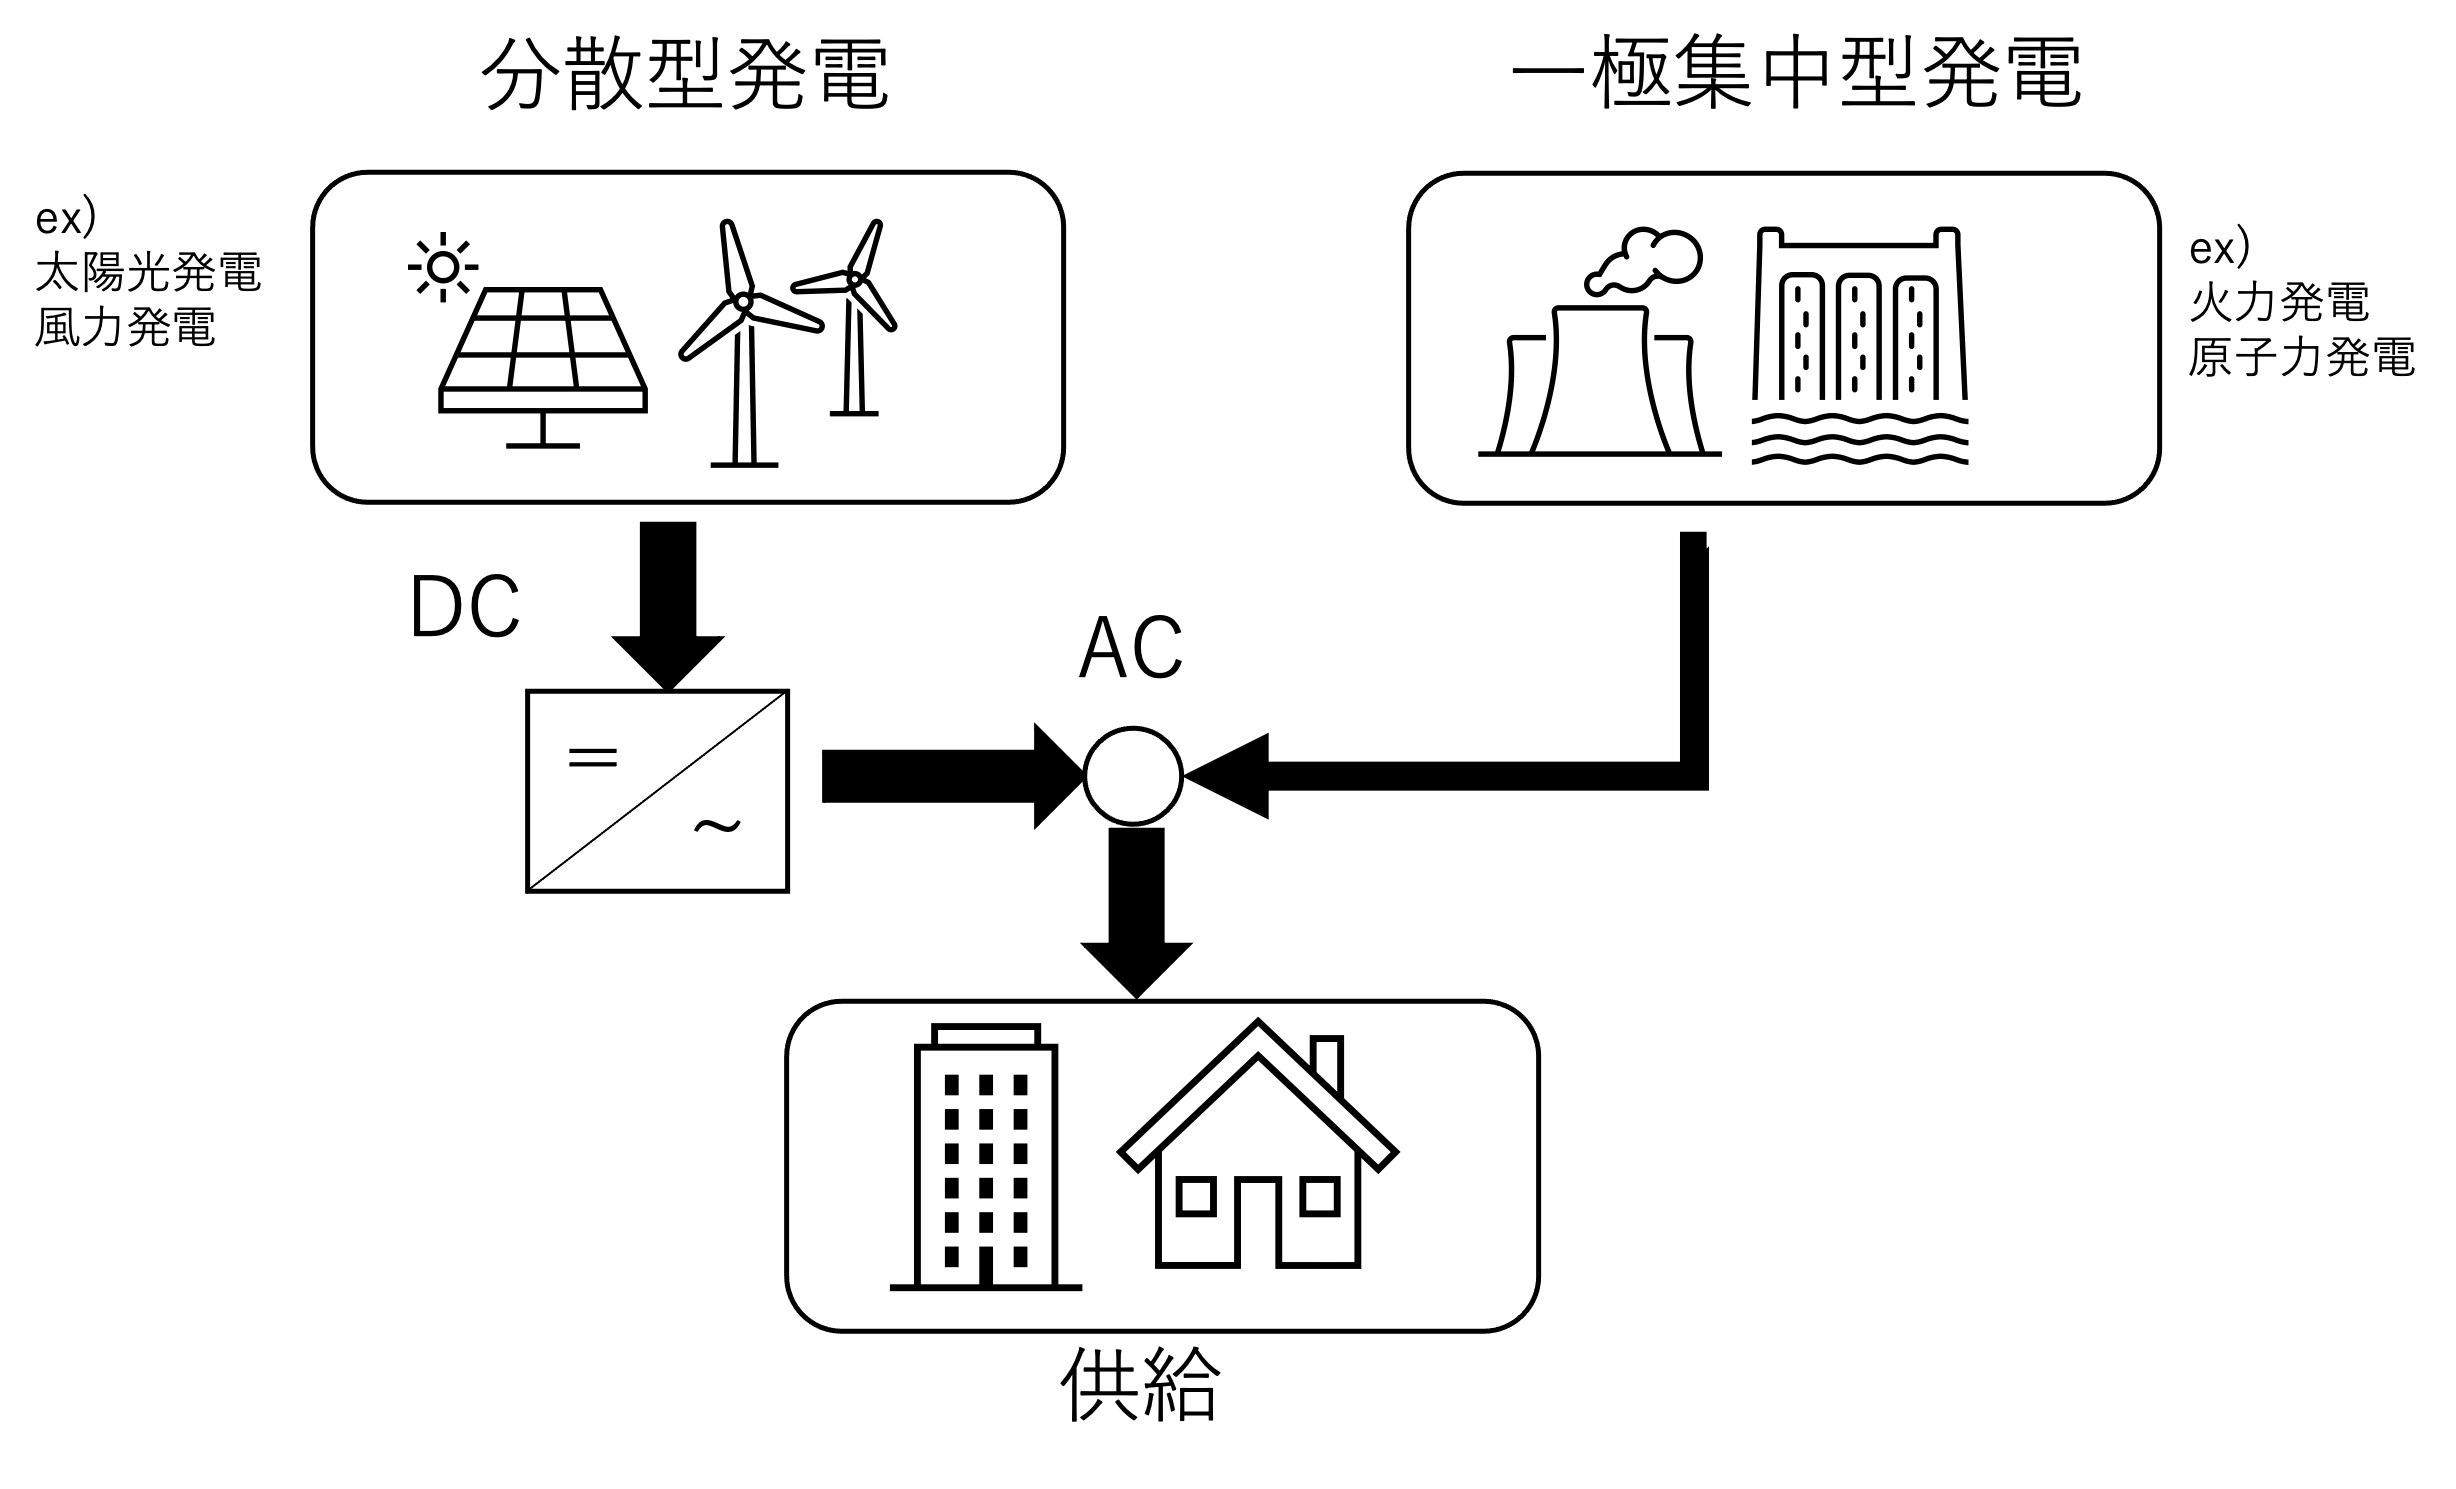
\includegraphics[width=140mm]{image/chapter1/Fig1.2.png}
    \caption{系統連系のイメージ図}
    \label{Fig1.2}
\end{figure}

現在では，分散型発電システムの需要拡大の観点から大容量な分散型発電システムの利用が進んでいる.電力容量が大容量になるにつれて接続される商用系統が高圧となり，従来のように系統電圧の情報をセンサで取得する場合，高価なセンサが必要となることや配線が複雑となるという問題がある.また，研究対象となる大規模太陽光発電システムについて，製品として提供しているものに連系リアクトル相当の配電盤は含まれておらず，配電盤は各需要家に存在するものであるため，連系リアクトルの値にばらつきが生じ，かつ系統電圧の情報をセンサから取得することが困難である.このことから，先行研究では大規模太陽光発電システムについて，連系リアクトルの値に依存しない制御手法の研究を行っていた．

\subsection{系統連系規定}
図\ref{Fig1.3}にFRT要件の一部事例を示す．
系統連系システムでは，分散型電源システム側で広範囲の瞬時電圧の低下や大規模電源脱落，周波数変動が発生した場合においても継続運転が可能となるために事故時運転継続要件(FRT:Fault Ride Through)を満たすシステムであることが求められている．この規定は日本電気技術企画委員会(JESC:Japan)により制定されている．

\newpage
\begin{figure}[ht]
    \center
    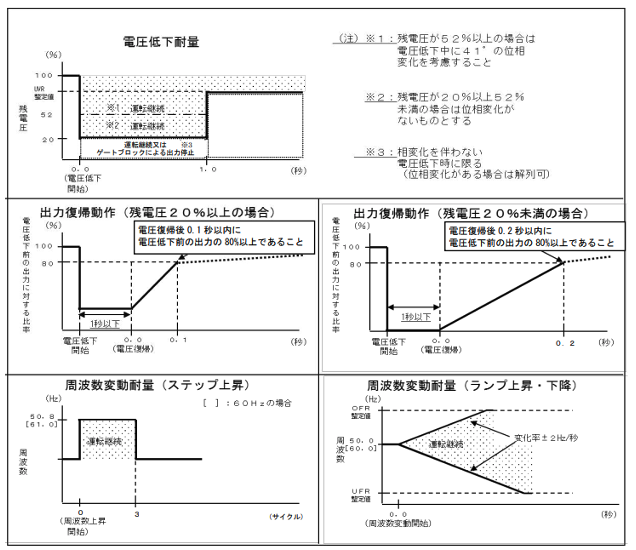
\includegraphics[width=140mm]{image/chapter1/Fig1.3.png}
    \caption{FRT要件の一部事例}
    \label{Fig1.3}
\end{figure}

FRT要件では，系統事故が発生し，系統電圧が20\%以下まで低下してもパワーコンディショナーのインバータを継続運転させて電力を供給する必要があり，系統電圧の低下立によって系統電圧復帰後にインバータの出力を80\%以上に戻すための許容時間が異なる．系統送電事故による広範囲の瞬時電圧低下・瞬時周波数上昇，大規模電源脱落，系統分離による周波数分離により，一斉解列や出力低下継続などが発生した場合，系統全体の電圧，周波数維持に大きな悪影響を及ぼす可能性があるため，パワーコンディショナーには事故発生時にも継続運転可能な高い制御性能が求められる．


%\newpage
\section{研究目的}
当研究室では，三角関数の積差の公式を用いて直交座標変換を行い，位相，振幅を算出する疑似dq変換を用いたPLL制御を提案している．
疑似dq変換はサンプリング周波数が高くなるとノイズの影響を受けやすくなり，検出精度が悪化してしまう．
これに対し，サンプリング周波数の異なる疑似dq変換回路を3並列化することでノイズの影響を低減している．
本研究では，ノイズ成分が相互に低減されるサンプリング周波数の組み合わせを探索し，
PLL制御の制御特性の向上を目的とする．\\
　疑似dq変換は系統電圧に対しての近似微分であるため，系統に低次高調波が含まれた場合に大きく動脈
してしまう．この課題に対し，複素係数フィルタを用いて系統電圧の瞬時複素ベクトルを容易
に算出し，なおかつ，優れた高調波外乱に対する耐性を有したPLL制御が提案されている\cite{ref03}．
複素係数フィルタを用いたPLL制御の初期検討として，複素係数フィルタの制御特性について検証する．